We now consider the extension of the results presented in Sec.~\ref{ch:penrose_binaries:sec:mp_penrose} to a binary system of rotating black holes described by the CMMR metric. In Weyl's cylindrical coordinates, the CMMR line element reads
%
\begin{multline}
  \ud s^2 = -f(\rho,z)\left[\ud t - \omega(\rho,z)\ud\phi\right]^2 \\
  + f(\rho,z)^{-1}\left[e^{2\gamma(\rho,z)}\left(\ud \rho^2 + \ud z^2\right) + \rho^2\ud\phi^2\right],
  \label{eq:cmmr_line_element}
\end{multline}
%
where the real valued functions $f(\rho,z)$, $\omega(\rho,z)$ and $\exp[2\gamma(\rho,z)]$ are defined as in Sec.~IV of Ref.~\cite{manko_ruiz_thermo}. As in the case of the MP metric, only the exterior of the black holes is described by these coordinates. In particular, the outer event horizons of the constituent black holes are straight lines in these coordinates (see Fig.~\ref{fig:cmmr_ergospheres}).

The CMMR solution is fully characterized by five independent parameters, namely the masses $M_{1,2}$, the angular momenta per unit mass $a_{1,2}$ and the coordinate distance $R$ between the black hole centers. From these, we define three additional parameters, namely $M_T = M_1 + M_2$, which represents the total mass of the system, $J_T = M_1 a_1 + M_2 a_2$, which represents the total angular momentum of the system, and $a_*$, which is a root of the cubic equation
%
\begin{equation}
  \left(R^2 - M_T^2 + a_*^2\right) \left(a_1 + a_2 - a_*\right) + 2 \left(R + M_T \right)\left(J_T - M_T a_* \right) = 0.
  \label{eq:cubic_eq_for_a}
\end{equation}

We note that, depending on the parameters, the CMMR metric can represent a black hole-black hole binary, a naked singularity-naked singularity binary, or a black hole-naked singularity binary~\cite{cabrera_metric,manko_ruiz_metric, manko_ruiz_thermo}. In our analysis, the chosen parameters always correspond to a binary black hole solution. In practice, this means that the chosen parameters must:
%
\begin{enumerate}
  \item Produce real valued and positive horizon lengths. The horizon half-lengths are given by the expressions $\sigma_1$ and $\sigma_2$ in Sec.~IV of Ref.~\cite{manko_ruiz_thermo}.
  \item Produce horizons that do not touch or overlap.
  \item Produce a single real root for $a_*$ in Eq.~\eqref{eq:cubic_eq_for_a}.
\end{enumerate}

\subsection{Geodesics}

Once again, we will make use of the Lagrangian formalism to determine the geodesic equations and the conserved quantities corresponding to the symmetries of the system. The Lagrangian associated with the geodesic motion of a massive and neutral test particle in the CMMR metric is~\cite{Dubeibe2016}
%
\begin{equation}
  2\mathcal{L} = -f(\dot{t} - \omega\dot{\phi})^2 +f^{-1}\left[e^{2\gamma}\left( \dot{\rho}^2 + \dot{z}^2 \right) + \rho^2\dot{\phi}^2 \right],
  \label{eq:cmmr_lagrangian}
\end{equation}
where, once again, dots represent derivatives with respect to the proper time $\lambda$.

%
Due to the stationarity and the axisymmetry of the system, we can identify two constants of the motion analogous to the quantities defined in Eqs.~\eqref{eq:conserved_energy}  and \eqref{eq:conserved_momentum}. The energy per unit mass, as measured by a static observer at infinity, is given by
%
\begin{equation}
  E = f\dot{t} - \omega f\dot{\phi},
  \label{eq:cmmr_energy_t_phi}
\end{equation}
%
and the angular momentum (with respect to the $z$ axis) per unit mass, as measured by a static observer at infinity, is given by
%
\begin{equation}
  L = \omega f \dot{t} + \left( \frac{\rho^2}{f} - \omega^2 f \right)\dot{\phi}.
  \label{eq:cmmr_ang_mom_t_phi}
\end{equation}
%

Using Eqs.~\eqref{eq:cmmr_energy_t_phi} and \eqref{eq:cmmr_ang_mom_t_phi} to eliminate $\dot{t}$ and $\dot{\phi}$ from the normalization of the four velocity, i.e. $\dot{x}^\mu\dot{x}_\mu = -1$, we obtain an expression for the energy $E$ in  terms of $\dot{\rho}$, $\dot{z}$ and the angular momentum $L$:
%
\begin{align}
  E  = & \frac{-f^2\omega L}{\rho^2-\omega^2 f^2}  + \left[ \frac{\rho^2e^{2\gamma}(\dot{\rho}^2 + \dot{z}^2)}{\rho^2 - \omega^2f^2}  \right. \nonumber \\
       & \left. + \left( \frac{\rho fL}{\rho^2 - \omega^2f^2} \right)^2 + \frac{\rho^2f}{\rho^2 - \omega^2f^2} \right]^{1/2},
  \label{eq:cmmr_energy_rho_z}
\end{align}
%
where the positive sign is once again chosen for the square root in order to guarantee that a static particle at infinity has positive energy. We rewrite the equation above as Eq.~\eqref{eq:effective1}, where the effective energy and the effective potential are now given by
%
\begin{equation}
  V_{\text{eff}} = \frac{\rho^2 - \omega^2 f^2}{\rho^2 e^{2\gamma}}\left[ \left( \frac{\rho fL}{\rho^2 - \omega^2f^2} \right)^2 + \frac{\rho^2f}{\rho^2 - \omega^2f^2}\right]
  \label{eq:cmmr_effective_potential}
\end{equation}
%
and
%
\begin{equation}
  E_{\text{eff}} = \frac{\rho^2 - \omega^2 f^2}{\rho^2 e^{2\gamma}}\left(E + \frac{f^2\omega L}{\rho^2-\omega^2 f^2}\right)^2.
  \label{eq:cmmr_effective_energy}
\end{equation}
%
%
Note that the constraints given in Eq.~\eqref{eq:effective_constraints} also apply to Eqs.~\eqref{eq:cmmr_effective_potential} and \eqref{eq:cmmr_effective_energy}.

The geodesic equations, analogous to Eqs.~\eqref{eq:ode_for_rho_motion} and \eqref{eq:ode_for_z_motion}, can be derived from the Euler-Lagrange equations for the Lagrangian \eqref{eq:cmmr_lagrangian}. Their explicit forms, in terms of $E$, $L$ and the metric functions $f$, $\omega$ and $e^{2\gamma}$, are given in Eqs.~(16) and (17) of Ref.~\cite{Dubeibe2016}. Once $\rho(\lambda)$ and $z(\lambda)$ are known, $t(\lambda)$ and $\phi(\lambda)$ are determined by direct integration of Eqs.~\eqref{eq:cmmr_energy_t_phi} and \eqref{eq:cmmr_ang_mom_t_phi}.


\subsection{Ergosphere}

Since the CMMR metric is stationary, and we are considering neutral particles in geodesic motion, we use the standard definition of an ergosphere to study the possibility of negative energy orbits and energy extraction. In other words, the ergosphere is the region where the time translation Killing vector field becomes space-like, i.e.~$(\partial_t)^\mu (\partial_t)_\mu > 0$. Taking into account the line element \eqref{eq:cmmr_line_element}, it is straightforward to show that the ergosphere of the CMMR spacetime is the locus of points that satisfy
%
\begin{equation}
  f(\rho,z) < 0.
  \label{eq:cmmr_ergo_ineq}
\end{equation}

We sketch this ergosphere in Fig.~\ref{fig:cmmr_ergospheres}, where each panel is labeled by a letter (\textbf{A}-\textbf{I}) and corresponds to a different set of parameters (which are specified in Table \ref{tab:cmmr_ergo_tab}). In each panel, the blue shaded region represents the $\phi = 0$ section of the ergosphere, while the red lines represent the event horizons of the black holes. The top row of the figure (panels \textbf{A}-\textbf{C}) exhibits the effect of changing the mass ratio of the system while keeping the total mass, both spins and the separation parameter fixed. It shows that, analogously to the MP case, initially disjoint ergospheres may merge into a single connected ergosphere when the mass ratio increases. The middle row of Fig.~\ref{fig:cmmr_ergospheres} (panels \textbf{D}-\textbf{E}), on the other hand, shows the effect of changing the spin parameter of the top black hole while keeping all other parameters fixed. We observe that when initially aligned spins become anti-aligned, the ergosphere becomes thinner and elongated along the symmetry axis. Finally, the bottom row (panels \textbf{G}-\textbf{H}) illustrates the effect of increasing the separation parameter when all other parameters are kept fixed. Similarly to what happens in the MP case, if the distance between the black holes is sufficiently large, there will be two disconnected ergospheres, one for each black hole.

\begin{figure}[!ht]
  \centering
  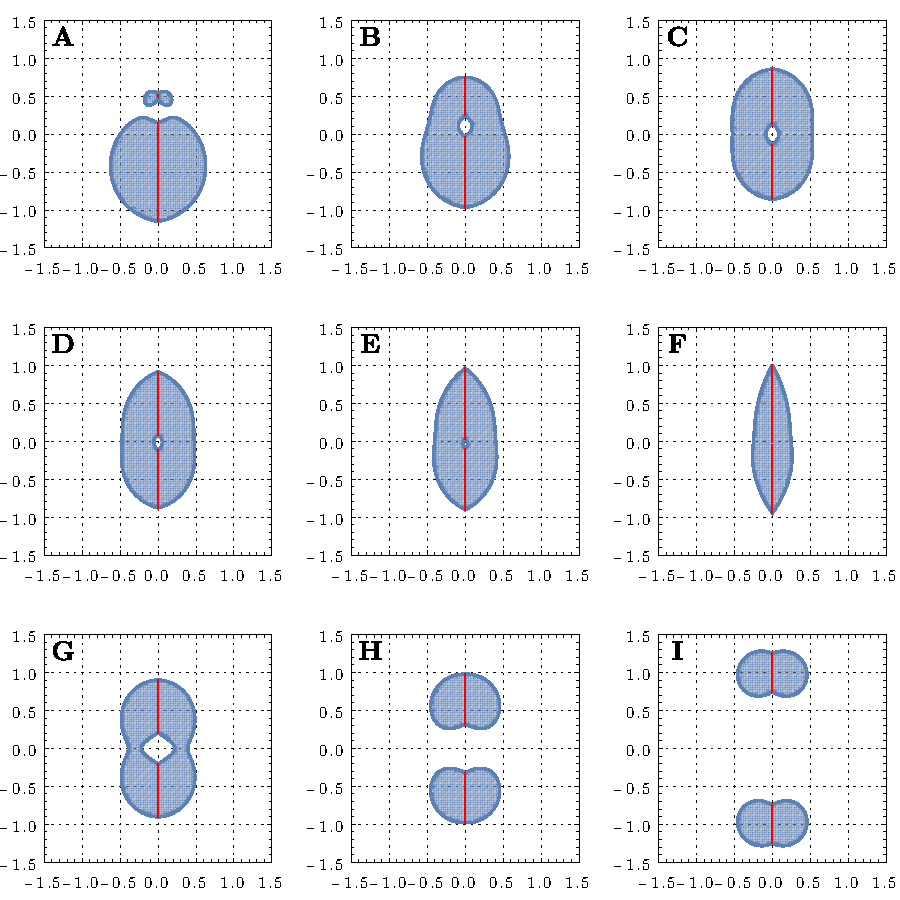
\includegraphics[width=\linewidth]{img/penrose_binaries/fig12.pdf}
  \caption{The $\phi=0$ section of the ergosphere of the CMMR metric for different set of parameters labeled \textbf{A}-\textbf{I} (see Table  \ref{tab:cmmr_ergo_tab}). In each plot the horizontal and vertical axes are $\rho/M_T$ and $z/M_T$, respectively. The red lines indicate the location of the black hole's horizons.}
  \label{fig:cmmr_ergospheres}
\end{figure}

\begin{table}[h]
  \centering
  \begin{tabular}{ccccc}
    \hline\hline
    Panel      & $M_1/M_2$ & $a_1/M_T$ & $a_2/M_T$ & $R/M_T$ \\
    \textbf{A} & $0.16$    & $0.65$    & $0.65$    & $1.00$  \\
    \textbf{B} & $0.58$    & $0.65$    & $0.65$    & $1.00$  \\
    \textbf{C} & $1.00$    & $0.65$    & $0.65$    & $1.00$  \\
    \textbf{D} & $1.00$    & $0.50$    & $0.65$    & $1.00$  \\
    \textbf{E} & $1.00$    & $0.30$    & $0.65$    & $1.00$  \\
    \textbf{F} & $1.00$    & $-0.10$   & $0.65$    & $1.00$  \\
    \textbf{G} & $1.00$    & $0.65$    & $0.65$    & $1.11$  \\
    \textbf{H} & $1.00$    & $0.65$    & $0.65$    & $1.30$  \\
    \textbf{I} & $1.00$    & $0.65$    & $0.65$    & $2.00$  \\
    \hline\hline
  \end{tabular}
  \caption{Parameters that define the CMMR metrics associated with the ergospheres \textbf{A}-\textbf{I} shown in Fig.~\ref{fig:cmmr_ergospheres}.}
  \label{tab:cmmr_ergo_tab}
\end{table}


\subsection{Bound negative energy orbits and the Penrose Process}

To demonstrate the existence of bound negative energy orbits and the possibility of using them to extract energy from non-coalescing Kerr binaries, we shall restrict our attention to systems of equal mass and spin. This symmetry allows for the existence of stable orbits (in the sense already discussed for the MP metric) in the $z=0$ plane. To find a negative energy trajectory that is confined outside the black holes, we choose the energy $E$ and the angular momentum $L$ such that there are two orbital turning points of Eq.~\eqref{eq:effective1} that lie inside the ergosphere of the system. Similarly to what was done in the MP case, once the initial radius $\rho(0)$, the energy, and the angular momentum are fixed, we solve Eq.~\eqref{eq:cmmr_energy_rho_z} to determine $\dot{\rho}(0)$ and integrate the geodesic equations. Using the parameters that produce the ergosphere \textbf{C} of Fig.~\ref{fig:cmmr_ergospheres} and Table \ref{tab:cmmr_ergo_tab}, we show an example of such a negative energy orbit in Fig.~\ref{fig:cmmr_veff} (right panel). The corresponding effective potential and effective energy are also shown in Fig.~\ref{fig:cmmr_veff} (left panel).

\begin{figure}[!ht]
  \centering
  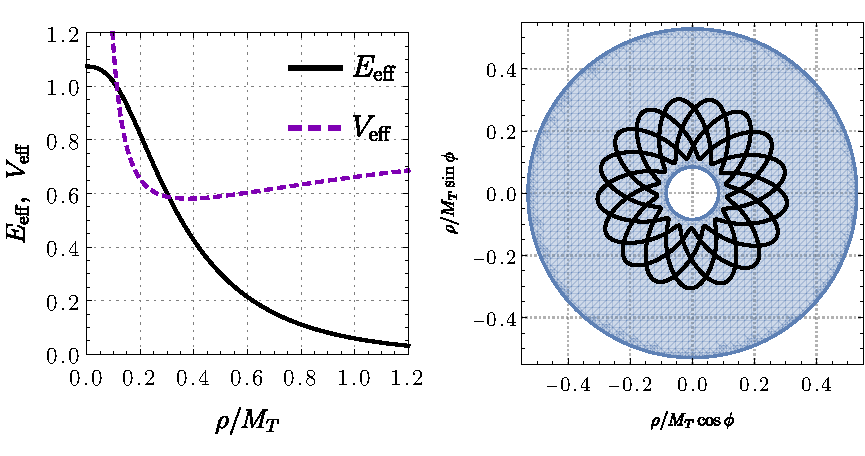
\includegraphics[width=\linewidth]{img/penrose_binaries/fig13.pdf}
  \caption{Left panel: effective energy (black curve) and effective potential (purple dashed curve) for $L=-2.5$ and $E=-0.054$, when the CMMR metric is characterized by $a_1=a_2=0.65$, $M_1 = M_2 = 0.5$, and $R = 1$ (corresponding to the label \textbf{C} in Table \ref{tab:cmmr_ergo_tab}). The turning points are located at $\rho_{-}/M_T = 0.112531$ and at $\rho_{+}/M_T = 0.306081$. Right panel: the associated trajectory in the $z = 0$ plane when $\rho(0)/M_T=0.25$ and $\phi(0)=0$. The blue region is the $z=0$ section of the ergosphere of the spacetime.}
  \label{fig:cmmr_veff}
\end{figure}

Adopting the same notation introduced Sec.~\ref{ch:penrose_binaries:sec:mp_penrose} for the trajectories in a Penrose process around the MP black hole, and taking advantage of the negative energy orbit depicted in Fig.~\ref{fig:cmmr_veff}, we now consider the possibility of energy extraction in the CMMR spacetime. By employing the conservation of 4-momentum (as in Sec.~III), we construct an explicit example of a Penrose process. The obtained trajectories are shown in Fig.~\ref{fig:cmmr_penrose} and the corresponding parameters are given in Table \ref{tab:cmmr_penrose_example}. The efficiency of the process, calculated through Eq.~\eqref{eq:penrose_efficiency_general}, is $\eta \approx 0.08 \%$.

\begin{figure}[!ht]
  \centering
  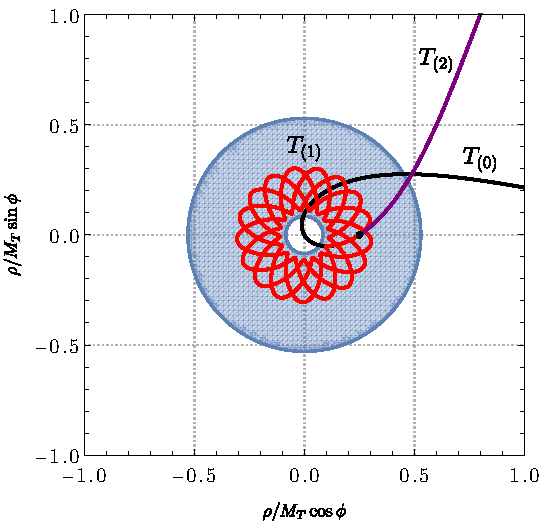
\includegraphics[width=\linewidth]{img/penrose_binaries/fig14.pdf}
  \caption{Penrose's process in the $z=0$ plane of a CMMR spacetime with $M_1=M_2=0.5$, $a_1=a_2=0.65$, and $R=1$. The incoming trajectory $T_{(0)}$ (black curve) splits at the black point ($\rho/M_T=0.25$, $\phi=0$) into the negative energy orbit $T_{(1)}$ (red curve) and the trajectory of the escaping fragment $T_{(2)}$ (purple curve). The parameters that generate these trajectories are shown in Table \ref{tab:cmmr_penrose_example}. The blue region is the $z=0$ section of the ergosphere (for particle 1).}
  \label{fig:cmmr_penrose}
\end{figure}

\renewcommand{\arraystretch}{1.2}
\begin{table}[h]
  \centering
  \begin{tabular}{ccccccc}
    \hline\hline
    $i$ & $m_{(i)}/m_0$ & $E_{(i)}$ & $L_{(i)}$         & $\dot{\rho}_{(i)}$ & $\dot{z}_{(i)}$ \\ \vspace{-0.3cm} \\
    0   & 1.0000000     & 2.00000   & 0         .000000 & 4.343904           & 0               \\
    1   & 0.0289697     & -0.05400  & -2.500000         & 0.313887           & 0               \\
    2   & 0.3148980     & 6.35623   & 0.229993          & 13.765800          & 0               \\
    \hline\hline
  \end{tabular}
  \caption{Parameters that generate the trajectories $T_{(0)}$, $T_{(1)}$, and $T_{(2)}$ of the Penrose process shown in Fig.~\ref{fig:cmmr_penrose}. The derivatives $\dot{\rho}_{(i)}$ and $\dot{z}_{(i)}$ are evaluated at the break-up point.}
  \label{tab:cmmr_penrose_example}
\end{table}